\hypertarget{fence-cid-resultados}{%
\section{Fluidez com integração contínua}\label{fence-cid-resultados}}

Desde a concepção da integração contínua para os repositórios \emph{Fate}, \emph{Fence} e \emph{Atlas} os \emph{pipelines} foram executados respectivamente e aproximadamente 350, 1000 e 2400 vezes, totalizando mais de 3750 execuções. Destas, 84\% obtiveram sucesso, 14\% falharam e o restante foi manualmente cancelada. Essas \emph{pipelines} foram responsáveis pela execução de mais 8 mil \emph{jobs} em uma duração média de 46 segundos para cada \emph{job} e mais de 100 horas totais. Isso tudo ocorreu nos últimos 4 meses, o que demonstra o quanto a integração contínua vem sendo utilizada pelos desenvolvedores do grupo.

O primeiro \emph{job} realizado pela maior parte das \emph{pipelines} do \emph{Fence CID} é o de \emph{build}. Este \emph{job} se certifica que o processo de compilação foi feito com sucesso e que a aplicação possui todos os recursos necessários. Em 6,4\% dos casos em que foi executado, foi identificado pelo menos um problema durante a compilação. Por conta dessas verificações, foi identificado a falta de padronização dentro do grupo em relação a preparação das dependências do software, assim como a não execução de alguns passos necessários para a compilação.

Geralmente presente seguidamente ao \emph{job} \emph{build}, existem os \emph{jobs} de testes unitários e de \emph{e2e}. Estes \emph{jobs} são os que mais encontram problemas quando executados, apresentando uma taxa de 14,6\% de identificação de falhas. Esta taxa corresponde a 70,4\% da acusação total de erros por \emph{jobs}, sendo o principal agente em alertar problemas com a nova versão da aplicação. Dada a eficiência destes testes, além do incentivo em aumentar a sua quantidade, há o interesse em investir também em outros tipos de testes e acrescentá-los à integração contínua, como os testes de integração.

É encontrado também em certos casos o \emph{job} de \emph{deploy}, que após a execução dos \emph{jobs} de \emph{build} e testes realiza a entrega da nova versão em uma máquina hospedeira. Fazendo parte da entrega contínua do \emph{Fence CID}, poucas falhas são identificadas por esse \emph{job}, sendo geralmente problemas existentes na máquina hospedeira. O maior benefício notado por esta implementação foi a automação e rapidez em disponibilizar uma nova versão em ambiente \emph{stage}. Para trabalho futuro seria interessante implementar também um \emph{deploy} automático para a máquina de produção, reduzindo as chances de falha humana.

A figura \ref{fig:testes-resultados} possui as comparações mais relevantes em relação aos resultados dos \emph{jobs}. A maior parte das tarefas são executadas para sistemas \emph{Atlas}, pois atualmente é o repositório com maior atividade dado ao maior número de desenvolvedores. Como existem tarefas para testes unitários e testes \emph{e2e}, os \emph{jobs} de testes são os mais executados pelo \emph{Fence CID}, e a detecção de falhas pelas tarefas de testes é consideravelmente superior à de outras tarefas. É possível observar também na figura o total de resultados obtidos com a execução dos \emph{jobs}.

\begin{figure}[H]
    \centering
    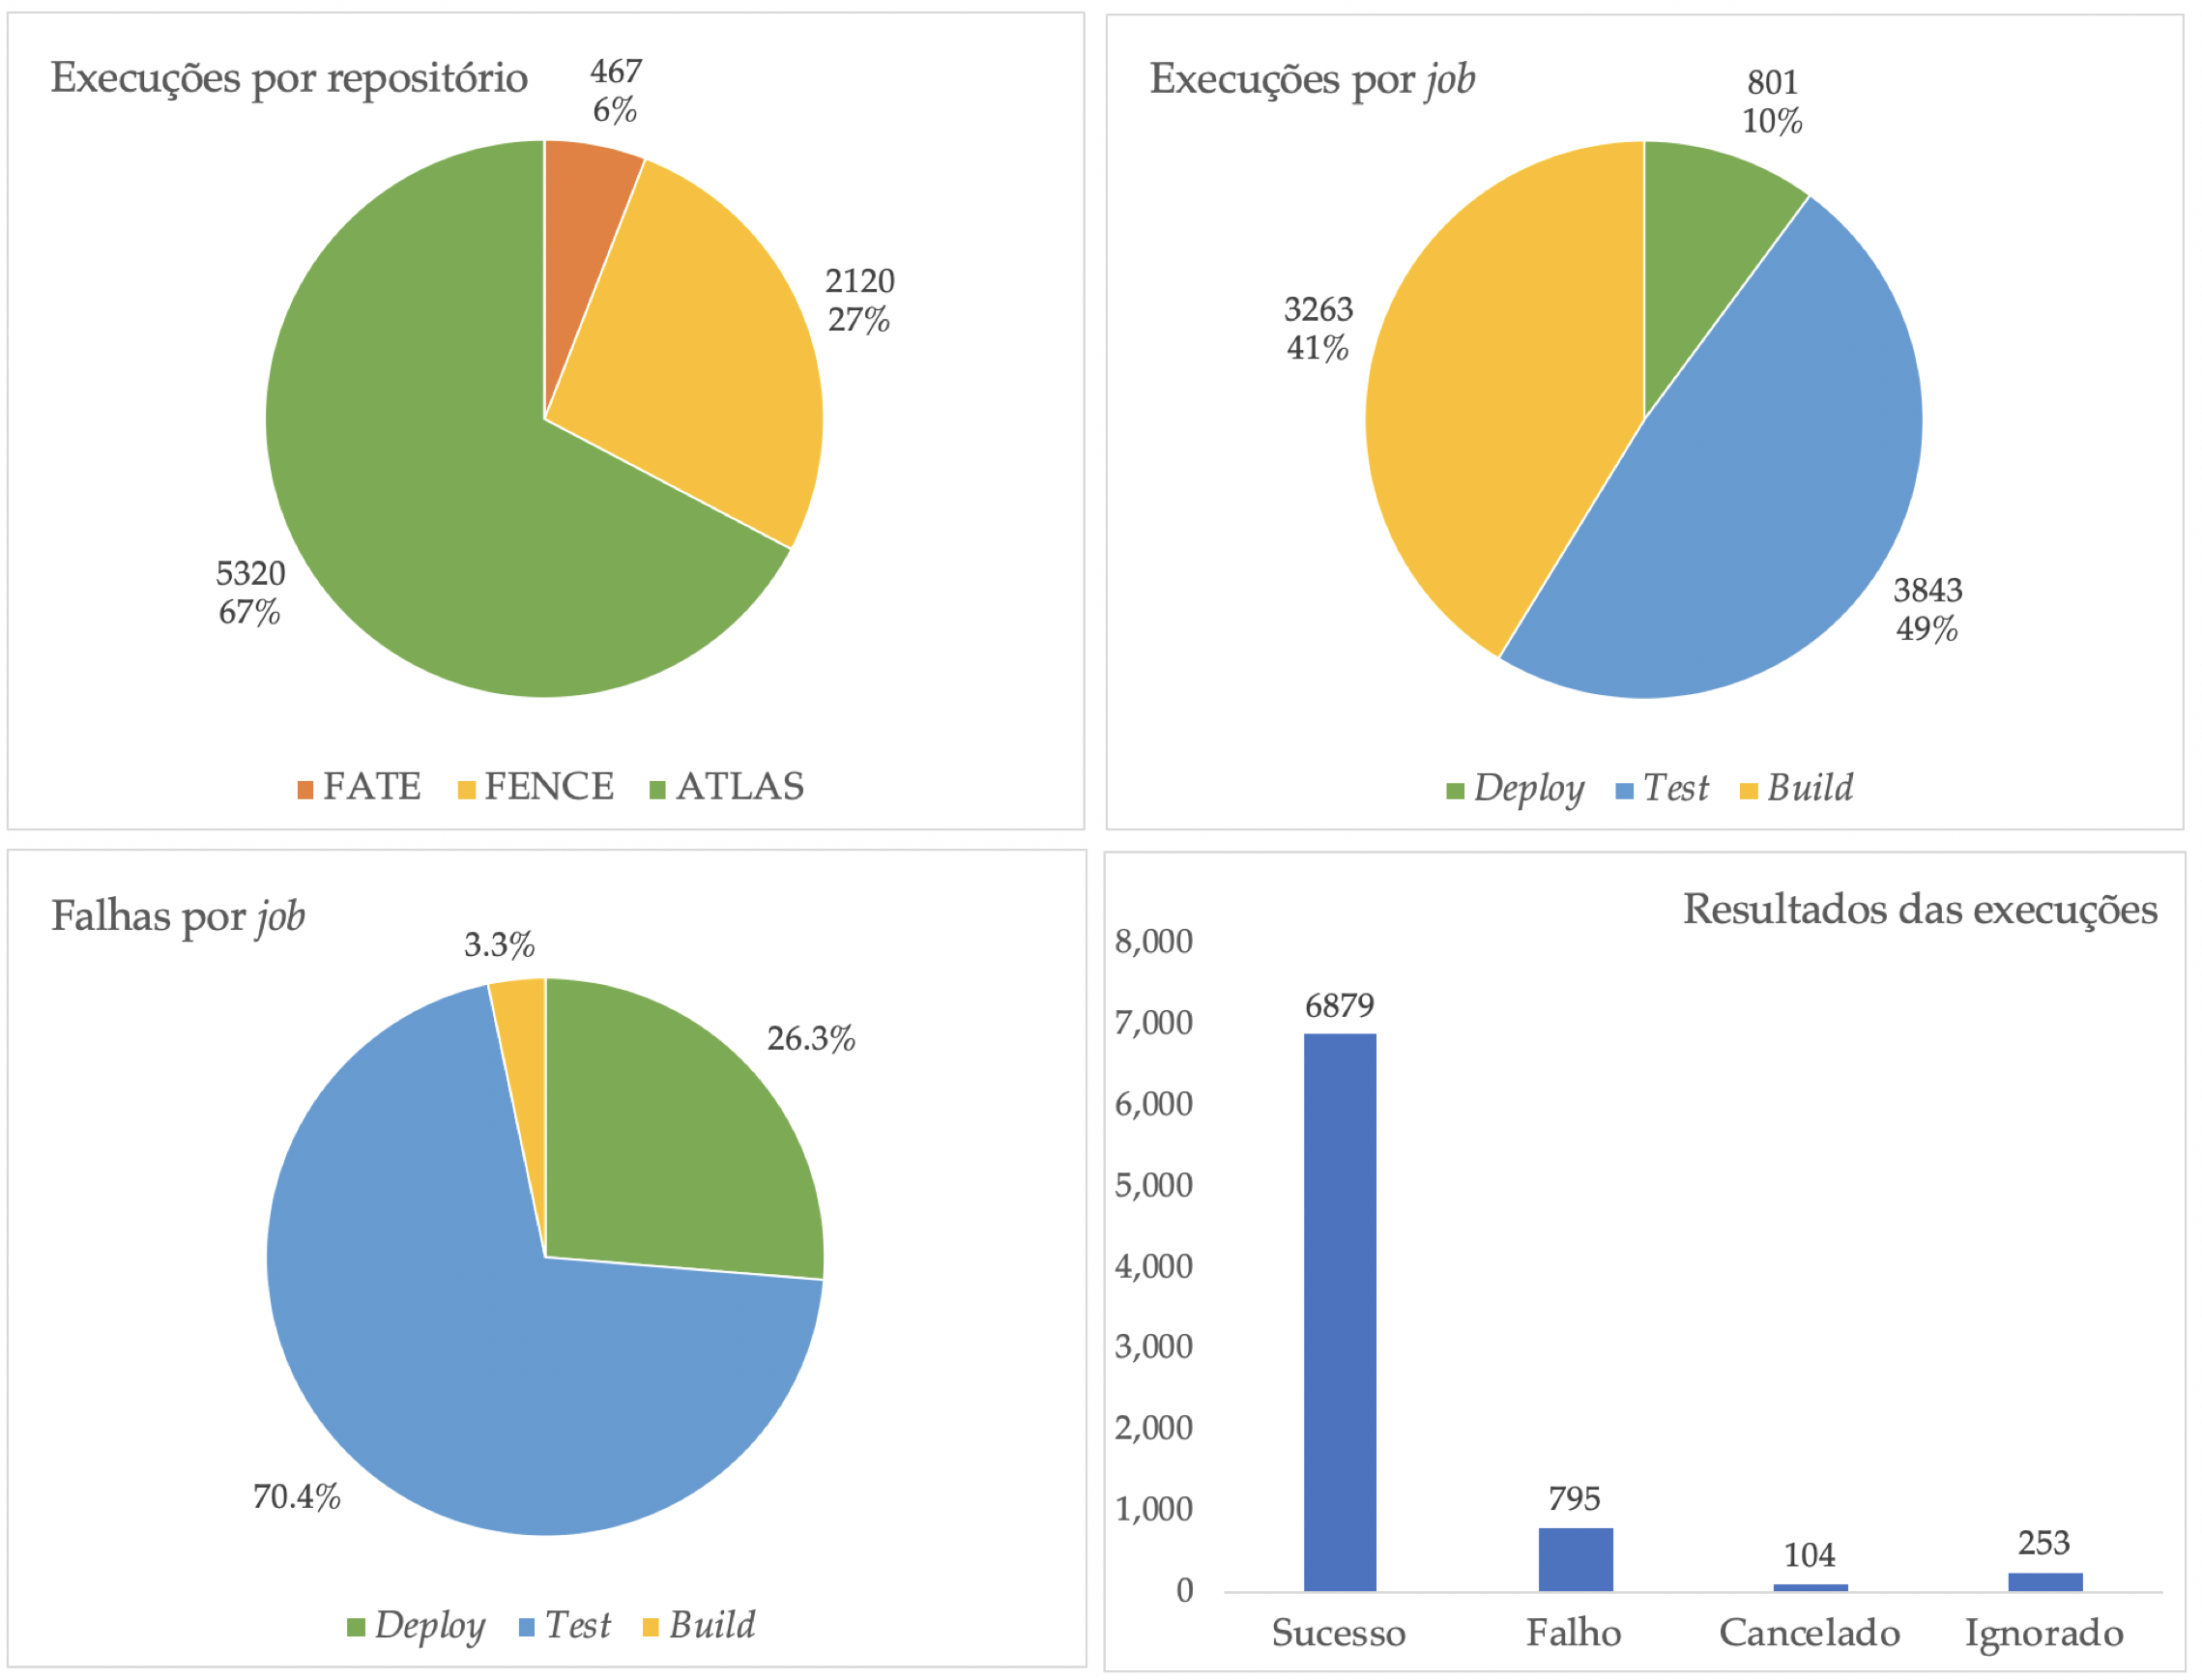
\includegraphics[width=15cm]{source/5-resultados/images/testes-resultados.png}
    \caption{Diversas comparações entre as execuções de \emph{job}.}
    \label{fig:testes-resultados}
\end{figure}

As vantagens trazidas pelo \emph{Fence CID} com a integração e entrega contínua justificam o esforço realizado em implementá-lo. O custo de manutenção é minimizado, sendo apenas necessário realizar alterações em arquivos de configuração. A ferramenta também provou estabilidade, executando a \emph{pipeline} em todos os momentos esperados, e eficiência, mantendo um baixo tempo de execução das tarefas.
